\section{Sun, Jul 15, 2018}

Been working on some things as of late. Nothing too
important mind you. Just some interesting things. There's
a section of the LDS Narrative which isn't in use anymore.
It's called the Journal of Discourses. The LDS Church no
longer confirms these as valid resources. So I started to
compile places where they've been used.

It was quite boring actually. But when the church controls
the narrative, they decide what is used and what isn't used as
can be expected. So yeah, it got boring. \ref{fig:jod} Shows
what they look like.

\begin{figure}[h!]
  \centering
  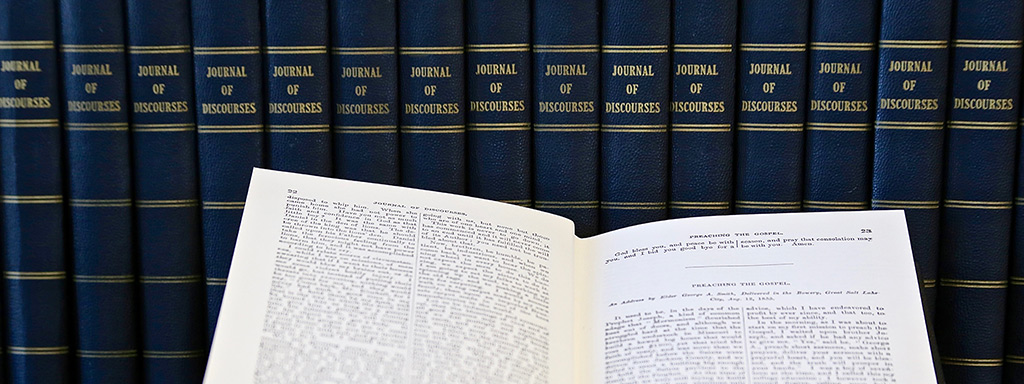
\includegraphics[width=1.0\linewidth]{2018/images/jod.jpg}
  \caption{Journal of Discourses}
  \label{fig:jod}
\end{figure}

There comes a time in life when you begin to realize things you 
were taught aren't exactly true. That's life right? Is that how
this life works somedasys? If it is? That doesn't feel like it
should be experienced that way. Life shouldn't be difficult. It's
meant to be joyful. Joy is a good thing to be found in life. It's
not always difficult or hard. It can't always be that way. Yes,
we have agency to do as we please. But there are consequences to
such a life aren't there? Aren't there options we can decide upon
to go through? Something like that.